%%%%%%%%%%%%%%%%%%%%%%%%%%%%%%%%%%%%%%%%%%%
%%%%%%  STYLE 24
%%%%%%%%%%%%%%%%%%%%%%%%%%%%%%%%%%%%%%%%%%%
\clearpage
\cxset{
 name=Chapter,
 numbering=arabic,
 number font-size=\Large,
 number font-family=\sffamily,
 number font-weight=\normalfont,
 number before={},
 number after={\space},
 number position=rightname,
 chapter font-family=\sffamily,
 chapter font-weight=\normalfont,
 chapter font-size=\Large,
 number after={},
 number dot=,
 chapter before={},
 chapter after={\par\thinrule\vskip12pt},
 chapter color={black!90},
 number color=\color{black!90},
 title beforeskip={},
 title afterskip={\vspace{30pt}},
 title before=,
 title after={\par},
 title font-family=\sffamily,
 title font-color=\color{black!80},
 title font-weight=\bfseries,
 title font-size=\LARGE,
 title afterskip=\par\vspace*{3cm}\thinrule\par\bigskip\bigskip}
\chapter{Introduction to style twenty four}

\def\objectives@{
\begin{tcolorbox}[width=\linewidth,boxsep=10pt,right=10pt]
\textbf{Learning Objectives}}
\def\stopobjectives@{\end{tcolorbox}}
\newenvironment{objectives}{\bigskip\objectives@}{\stopobjectives@\bigskip}

\begin{objectives}
\par
\lipsum[1]
\bigskip\bigskip
\end{objectives}

This design is ideal for scholarly books or notes. It has a nice clean design with a shaded block for the learning objectives.
\medskip
\begin{figure}[ht]
\centering
\fbox{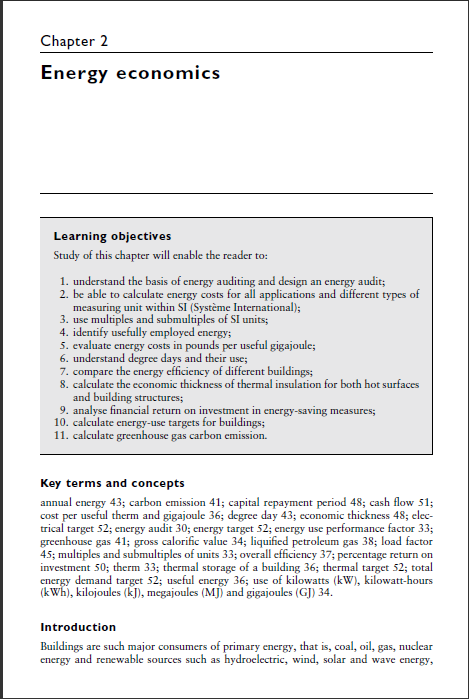
\includegraphics[width=0.6\textwidth]{./chapters/chapter24}}
\end{figure}
\lipsum[2-3]

